\documentclass[10pt]{article}
\usepackage[T1]{fontenc}\usepackage{lmodern,amsmath,amssymb,graphicx,hyperref}
\usepackage[margin=.75in]{geometry}
\setlength{\parindent}{0pt}\setlength{\parskip}{7pt}
\begin{document}
\begin{center}{\Large Full retained crossing content}\\[4pt]
Actual paired construction --- 16 November 2026\end{center}
\textbf{The complete matrix bound.} Set $a=u+1$, use the same previously
constructed multiplicities $m_j=4\,\mathrm{profile}(u,j)$, and keep the actual
source grid. Write $D(T)=W_{00}(T)$ and let $\pi$ flip the high bit while
preserving the lower $u$ bits. The actual anchor weight is
\[
 U_x=\prod_{j<u}\left(\frac{2^j}{2^j-\delta(x,\pi x)}\right)^{m_j}.
\]
The already constructed origin $S$ has entries $S_{x,\pi x}=-U_x$ and zero
elsewhere. Both $S$ and its inverse are integral. Define
$K=W+D(S-I)$ as in the previous checkpoint [pcc:unverified].

For \emph{every} original nonzero grid node $t$ with $v_2(t)=i<u$, and every
crossing pair $x_i=y_i$, local148/receipt080 establishes
\[
 \operatorname{Content}_{u-i}
 \left(c_i^{-1}\,K_{xy}(t+\alpha Z)\right),\qquad
 c_i=\operatorname{diagonalJet}(u+1,u,i,m),\quad \alpha=2^{u+2}.
\]
Here Content means every rational polynomial coefficient is zero or has
valuation at least its subscript. It is not a first-jet or numerical-rank
statement. The fixed $c_i$ is the already known nonzero negative-pole
normalizer, never a potentially vanishing derivative at $t$
[pcc:unverified].

Undoing that normalization gives the absolute bound
\[
 \operatorname{Content}_{w+u-i}K_{xy}(t+\alpha Z),\qquad
 w=\operatorname{jetWeight}(u+1,u,i,m).
\]
The old exact schedule is four, so $w=u+6-i$. Positive anchor nodes are
included; their vanishing local jets are allowed [pcc:unverified].

\textbf{Same objects and budget.} The multiplicity profile is unchanged.
The earlier explicit origin unit, exact nonzero-node values of $K$, and
old degree cap $|\mathrm{grid}|-1+\mathrm{mass}$ remain valid. No gain,
nonzero unit, rank or new multiplicity profile is supplied as a hypothesis.

\textbf{Evidence scope.} Local148 has50 source statements including45 parent
statements. Compiler exit0, no warnings, and standard printed central
dependencies are retained. This is local elaboration evidence, outside
shared Transport53/57 audit/fresh; producer records are unsigned and default
\texttt{not\_covered} [pcc:unverified].
\newpage
\begin{center}{\Large From exact pairs to all crossing entries}\end{center}
\textbf{Paired entries.} The exact prior polynomial identity is
\[
 (T-\delta)K_{x,\pi x}(T)=\delta D(T)U_x,
 \qquad \delta=\pm2^u.
\]
Local143 derives $v_2(t-\delta)=i$ for every nonzero integer $t$ of valuation
$i<u$. The normalized affine denominator is
\[
 E(Z)=1+\frac{\alpha}{t-\delta}Z,\qquad
 \operatorname{Content}_1(E-1).
\]
The displacement ratio $\delta/(t-\delta)$ has content $u-i$. Existing old
normalized-chart integrality and the actual integral $U_x$ give the initial
integrality and numerator bounds. Applying the existing
\texttt{content\_cancel\_near\_one} as stated yields the entire paired
polynomial content, local145/receipt078 [pcc:unverified].

\textbf{Other residues.} The actual schedule row implies
$\mathrm{profile}(u,j)\ge u-j$. At the first differing retained bit $s$,
apply the existing low-order or omitted-high gain theorem. Under the same
$m=4\,\mathrm{profile}$, either margin is at least $u-i$. Existing graded
base and correction bounds, and the actual zero constant coefficient,
give the full old normalized crossing content. These entries of $K$ equal
the old entries exactly, local147/receipt079 [pcc:unverified].

\textbf{No missing residue case.} At $a=u+1$, an actual lower-$u$ residue
class consists of self and its high-bit partner. Local148 derives this
classification from the actual block equivalence. The new diagonal is
identically zero, so all crossing entries are covered [pcc:unverified].
\begin{center}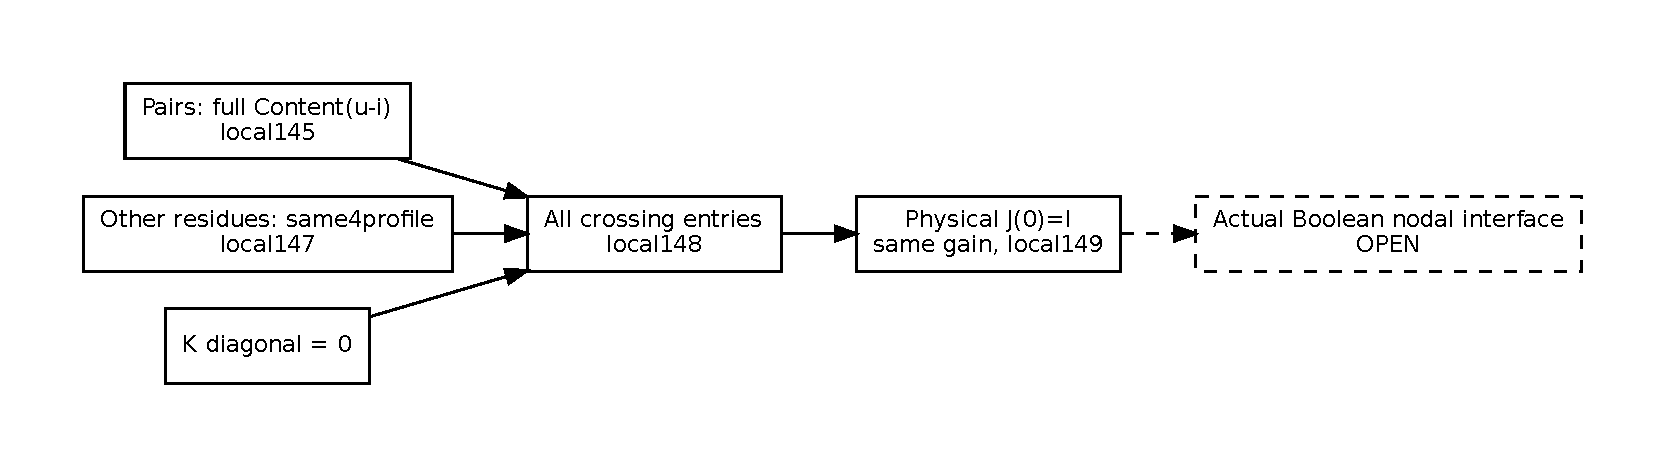
\includegraphics[width=.95\linewidth]{whole-crossing-dependencies-001.pdf}\end{center}

All nodes above refer to the same polynomial and same source grid. No
negative-pole-only test, favorable local unit, selected coefficient or
independence assumption replaces these statements. The ignored higher
valuation levels and original node/Boolean/recursion interface still need
their actual algorithmic treatment; this theorem does not waive them.
\newpage
\begin{center}{\Large Identity origin restored; Boolean interface remains}\end{center}
\textbf{Explicit physical normalization.} Define a single new physical
polynomial family by a weighted column permutation:
\[
 J_{xy}(T)=-U_y^{-1}K_{x,\pi y}(T).
\]
Local149/receipt081 establishes $J(0)=I$, unchanged degree and the same full
retained crossing content, since $\pi y$ retains bit $i<u$ and $U_y^{-1}$
is integral. Its nonzero node values change explicitly:
\[
 J_{xy}(t)=-U_y^{-1}W_{x,\pi y}(t),\qquad t\ne0.
\]
This is not a claim that every original node value is preserved, or that
$J-W$ has the old $C H$ form. Local149 has56 source statements including50
parent statements and six new endpoints, compiler exit0/no warnings
[pcc:unverified].

\textbf{A known invalid shortcut is excluded.} The actual original Boolean
kernel is
\[
 B(A)[Y,X]=\prod_j\ell_{Y_j}((A X)_j),\qquad
 \ell_0(z)=1-z,\quad\ell_1(z)=z.
\]
The repository's exact mod4 counterexample shows that physical matrix
composition does not generally imply $B(AB)=B(A)B(B)$. A physical inverse
therefore does not automatically supply a Boolean tensor gauge or the
original recovery interface. This restriction was checked against the
primary common-kernel README and Boolean-gauges review [pcc:unverified].

\textbf{Next decisive test.} Read the exact nodal Cauchy maps and original
attached tensors, then prove or refute the restricted composition needed
for these \emph{actual} partial-monomial nodal maps and this weighted
normalization. That possible restriction is prospective. A missing generic
law belongs in crypto-lean first. Carry the transformed tensors, finite
precision and nilpotent rings, both axes, immutable creation descriptions
and all preparation costs [pcc:unverified]. Resume \texttt{PROTOCOL-024.md}.

Entrywise content is not compact weighted-factor construction, mode
density, cheap recursive extraction or a complete expected bit-cost bound.
Those and the original elliptic relation/public-input finder and scalar
recovery remain separate obligations. No performance or algorithm conclusion
is promoted here [pcc:unverified].

\textbf{Preservation.} Failed142/144/146 and unrun141 are retained; all old
archives, reports, claim bodies and raw bytes remain unchanged. No new
native, timing, scaling or paid experiment was run. Standard algebra is
reused; novelty of an eventual application is unverified.
\end{document}
